\section{Grafo}
\label{sec:grafo}

Un grafo es un objeto matemático en el cual arcos conectan pares de vértices. Formalmente:

\begin{definicion}{Grafo}{grafo}
  Un \concept{grafo} $G$ es un par ordenado de conjuntos disjuntos $(V, E)$ tal que $V$ es un conjunto de \concept{vértices} o \concept{nodos} y $E$ es un conjunto de \concept{aristas} o \concept{arcos} que conectan pares de vértices.
\end{definicion}

Gráficamente, los vértices se representan por puntos y los arcos se representan por segmentos de recta que los conectan. El siguiente es un ejemplo de grafo donde cada vértice están marcado con una letra:

\begin{center}
  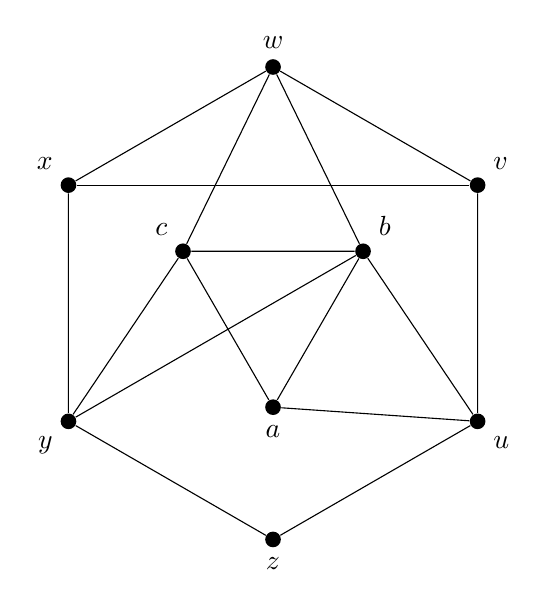
\begin{tikzpicture}[scale=1.2,
    vertex/.style={circle, fill=black, inner sep=2pt}]
    % Outer vertices (on c circle of radius 2.5)
    \node[vertex, label=above:$w$]      (w) at (90:2.5)  {};
    \node[vertex, label=above right:$v$](v) at (30:2.5)  {};
    \node[vertex, label=below right:$u$](u) at (330:2.5) {};
    \node[vertex, label=below:$z$]      (z) at (270:2.5) {};
    \node[vertex, label=below left:$y$] (y) at (210:2.5) {};
    \node[vertex, label=above left:$x$] (x) at (150:2.5) {};
    % Inner vertices (on c circle of radius 1.1)
    \node[vertex, label=above left:$c$] (c) at (150:1.1) {};
    \node[vertex, label=below:$a$]      (a) at (270:1.1) {};
    \node[vertex, label=above right:$b$](b) at (30:1.1)  {};
    % Outer cycle
    \draw (y)--(z)--(u)--(v)--(w)--(x)--(y);
    % Outer diagonal
    \draw (x)--(v);
    % Inner triangle
    \draw (c)--(b)--(a)--(c);
    % Outer-to-inner spokes
    \draw (w)--(c) (w)--(b);
    \draw (y)--(c) (y)--(b);
    \draw (u)--(b) (u)--(b);
    \draw (a)--(u);
  \end{tikzpicture}
\end{center}

En ocasiones es útil enfatizar que $V$ es el conjunto de vértices de $G$ escribiendo $V(G)$, para no confundirlo con un posible conjunto de vértices $V(H)$ del grafo $H$. Lo mismo se puede hacer para $E(G)$ y $E(H)$.

Salvo que explícitamente se diga lo contrario, en estos apuntes se estudian \concept{grafos finitos}, en los que los conjuntos $V$ y $E$ son finitos.
